% This is samplepaper.tex, a sample chapter demonstrating the
% LLNCS macro package for Springer Computer Science proceedings;
% Version 2.20 of 2017/10/04
%
\documentclass[runningheads]{llncs}
%
\usepackage{graphicx}
% Used for displaying a sample figure. If possible, figure files should
% be included in EPS format.
%
% If you use the hyperref package, please uncomment the following line
% to display URLs in blue roman font according to Springer's eBook style:
% \renewcommand\UrlFont{\color{blue}\rmfamily}
\usepackage{amsmath,amssymb}
\usepackage{amsfonts}

\begin{document}
%
\title{Deep Triplet Network adopting the Kernel and the Range Space Learning for Wi-Fi Handwritten Signature Verification}
%
\titlerunning{Triplet Network adopting KAR Learning for Wi-Fi Signature Verification}
% If the paper title is too long for the running head, you can set
% an abbreviated paper title here
%
\author{Young-Woong Kwon \and Jooyoung Kim \and Kar-Ann Toh}
%
\authorrunning{Y. Kwon et al.}
% First names are abbreviated in the running head.
% If there are more than two authors, 'et al.' is used.
%
\institute{
School of Electrical and Electronic Engineering, Yonsei University, 50 Yonsei-ro, Seodaemun-gu, Seoul 03722, Republic of Korea\\
\email{\{herokwon, harrykim, katoh\}@yonsei.ac.kr}}
%
\maketitle              % typeset the header of the contribution
%
\begin{abstract}
%The abstract should briefly summarize the contents of the paper in 15--250 words.
In this paper, we propose an identity verification system based on the handwritten signature signals captured by the Wi-Fi CSI signals using a triplet network. 
To refine the triplet inputs for faster loss convergence, the kernel and the range space learning is adopted to mine the distinctive triple inputs from the training set of Wi-Fi signature signals. 
Subsequently, the triplet network utilizing the ConvNet structure is trained with the mined triplet inputs based on L-2 distance comparison. 
Our experiments on an in-house Wi-Fi handwritten signature signal dataset show encouraging verification accuracy with faster training loss convergence comparing with the baseline triplet network and the Siamese network.

\keywords{Wi-Fi signature signal \and in-air handwritten signature verification \and the Kernel and the Range space projection learning \and triplet network}
\end{abstract}
%
%
%
\section{Introduction}

In recent years, several behavioral biometric traits for identity authentication are investigated since they are free from the physical characteristic which user owns~\cite{bailador2011analysis}. Among the behavioral biometrics, the signature based user authentication~\cite{galbally2015line,sanmorino2012survey} is taking considerable interest with the development of the in-air signature recognition systems~\cite{galbally2015line,jeon2012system,malik20183dairsig}. 
With the help of sensors such as a depth camera~\cite{malik20183dairsig} or mobile sensor~\cite{jeon2012system}, the in-air signature recognition systems could have less spatial limitation in the signature acquisition process compare to other contact-based authentication systems. 

Recently, the commercial Wi-Fi device is also proposed to be utilized as a in-air signature acquisition sensor due to its easy accessible property \cite{moon2017air}. By capturing the Wi-Fi CSI signal to observe the distinctive motions, the Wi-Fi based in-air signature recognition system showed reasonable user verification performance~\cite{moon2017air}. However, the previous works on Wi-Fi signal based user authentication systems~\cite{hong2016wfid,moon2017air} utilized the conventional feature extraction method such as the Principal Components Analysis. Since the conventional feature extraction method is not enough to extract the direction- or pose-invariant features from the acquired in-air data, more recently, some studies attempted to implement the deep learning algorithms in Wi-Fi signal based user authentication systems for the better verification performance ~\cite{shi2017smart,pokkunuru2018neuralwave}. 

In this paper, we utilize the deep triplet network for identity verification based on Wi-Fi CSI signature signal. To achieve not only the promising verification accuracy but also the fast training loss convergence speed for the commercial use, we adopt the kernel and the range (KAR) space leaning~\cite{toh100,toh2018learning,toh2018analytic,toh2018gradient} to mine the distinctive triplet inputs for training the triplet network. Subsequently, the triplet network utilizing the ConvNet structure as a feature extractor is trained using the mined triplet inputs based on L-2 distance comparison.
The main contributions of our work can be summarized as follows:
\begin{itemize}
\item Proposal of a system for identity verification based on the Wi-Fi handwritten signature signals using deep triplet network.
\item Adopted the KAR space learning to mine the distinctive triplet inputs which boosted the convergence speed of the training loss in triplet network.
\item Provision of the experimental study on an in-house Wi-Fi handwritten signature signal dataset collected from 50 subjects.
\end{itemize}

The paper is organized as follows: the related works including triplet network and KAR space learning will be introduced in Section 2 for immediate reference. Our proposed method will be discussed in Section 3. Section 4 describes our experimental results and analysis. Some concluding remarks will be followed in Section 5.


\section{Related Works}

\subsection{Triplet Network}
% metric learning
Metric learning is the training of models to learn a distance function to find similarities between objects. 
% triplet network
Triplet network a metric learning model which aims to learn useful representations by distance comparisons \cite{hoffer2015deep}. It is widely used in face recognition \cite{schroff2015facenet} and person re-identification, which solves the matching problem of individuals and identity between camera images\cite{cheng2016person,chen2017beyond}. In above tasks, distinction between classes may be ambiguous as the textures or features of the targets may be similar looking.

% training triplet network
Triplet network receives triplet data pairs as input. Triplet is composed of anchor(reference), positive(similar) and negative(dissimilar) data.
The training of the triplet network is making feature vectors to be placed in the appropriate separation space, making the positive(similar) data is close to the anchor(reference) and the negative(dissimilar) data is kept away from the anchor.
 
% optimize training
Since myriad triplet pairs may exist for the training set, training from all possible pairs may time-consuming and unnecessary. Optimizing training becomes necessary as it mines the learning-efficient triplet out of large possible inputs.
There are many ways to optimize training. In \cite{schroff2015facenet}, selects inputs from large mini-batch at each training iteration using the network during training. \cite{cheng2016person} adds second margin for triplet loss to expand intra-class distance.
Following in \cite{chen2017beyond}, quadruplet loss function makes the distance between the same classes is less than the distance between any different classes. 

% Rel works: KAR learning
\subsection{kernel and the range space learning}\label{kar}

The multilayer feedforward neural networks is generally trained by the gradient descent method and the backpropagation.
However, setting the learning parameters such as learning rate or momentum value is important to use the gradient descent method. 

Recently, gradient-free learning framework based on series of the kernel and the range (KAR) space manipulation has developed \cite{toh2018learning,toh2018gradient}.
Since it is trained by linear equations, no learning parameters nor the iteration are needed to train the networks.
Using this novel framework, we can train multilayer feedforward neural networks with any numbers and size of layers.

% Karnet structure and mining samples.
Let the training dataset $\mathbf{X}\in{\mathbb{R}}^{m \times (n+1)}$ and $\mathbf{G}\in{\mathbb{R}}^{m \times n}$ is network outputs.
Multilayer neural network structure is shown below:
\begin{equation}
    \mathbf{G} = \sigma\left(\left[\mathbf{1},\sigma\left(\dots\left[\mathbf{1},\sigma\left(\left[\mathbf{1},\sigma\left(\mathbf{X}\mathbf{W}_{1}\right)\right]\mathbf{W}_{2}\right)\right]\dots\mathbf{W}_{(i-1)}\right)\right]\mathbf{W}_{i}\right),
\end{equation}
where $\mathbf{W}_{1}\in{\mathbb{R}}^{(n+1) \times h_{1}}$,$\mathbf{W}_{2}\in{\mathbb{R}}^{(h_{1}+1) \times h_{2}}$,$\dots,\mathbf{W}_{i}\in{\mathbb{R}}^{(h_{(i-1)}+1) \times n}$,$\mathbf{1}=\left[1,\dots,1\right]^{T}\\
\in{\mathbb{R}}^{m \times 1}$ and $\sigma(.)$ is activation function.

% training KARnet
Network learning is archived using one-hot encoded target $\mathbf{Y}\in{\mathbb{R}}^{m \times n}$ instead of network output $\mathbf{G}$.
After that, we have the weight matrix $\mathbf{W}_{1}\dots\mathbf{W}_{i}$ to train. the weight matrix can be separated into weights and bias term as
$\mathbf{W}_{2}\dots\mathbf{W}_{i}$ = 
$\begin{bmatrix}
\mathbf{w}_{2}^{T}\\\mathnormal{W}_{2}
\end{bmatrix}
\dots
\begin{bmatrix}
\mathbf{w}_{i}^{T}\\\mathnormal{W}_{i}
\end{bmatrix}$.

after assign random weights to $\mathbf{W}_{1}\dots\mathbf{W}_{i}$ , we get $\mathbf{W}_{1}$. it is solved as follows:

\begin{equation*}
    \left[\sigma^{-1}\left(\mathbf{Y}\right)-\mathbf{1}\cdot\mathbf{w}_{i}^{T}\right]\mathnormal{W}_{i}^\dagger = 
    \sigma\left(\dots\left[\mathbf{1},\sigma\left(\left[\mathbf{1},\sigma\left(\mathbf{X}\mathbf{W}_{1}\right)\right]\mathbf{W}_{2}\right)\right]\dots\mathbf{W}_{(i-1)}\right)
\end{equation*}
\begin{equation*}
    \begin{aligned}
        \Rightarrow
        \biggl[\sigma^{-1}\biggl(
        \dots
        \biggl[\sigma^{-1}\biggl(
            \left[\sigma^{-1}\left(\mathbf{Y}\right)-\mathbf{1}\cdot\mathbf{w}_{i}^{T}\right]\mathnormal{W}_{i}^\dagger
        \biggr)
        - \mathbf{1}\cdot\mathbf{w}_{(i-1)}^{T}\biggr]\mathnormal{W}_{(i-1)}^{\dagger}
        \dots\biggr)\\
        - \mathbf{1}\cdot\mathbf{w}_{2}^{T}\biggr]\mathnormal{W}_{2}^{\dagger} 
        = \sigma\left(\mathbf{X}\mathbf{W}_{1}\right)
    \end{aligned}
\end{equation*}
\begin{equation}
    \begin{aligned}
        \Rightarrow
        \mathbf{X}^{\dagger}\sigma^{-1}\biggl(
        \biggl[\sigma^{-1}\biggl(
        \dots
        \biggl[\sigma^{-1}\biggl(
            \left[\sigma^{-1}\left(\mathbf{Y}\right)-\mathbf{1}\cdot\mathbf{w}_{i}^{T}\right]\mathnormal{W}_{i}^\dagger
        \biggr)
        - \mathbf{1}\cdot\mathbf{w}_{(i-1)}^{T}\biggr]\mathnormal{W}_{(i-1)}^{\dagger}
        \dots\biggr)\\
        - \mathbf{1}\cdot\mathbf{w}_{2}^{T}\biggr]\mathnormal{W}_{2}^{\dagger}
        = \mathbf{W}_{1} .
    \end{aligned}
\end{equation}

After deriving the $\mathbf{W}_{1}$, the $\mathbf{W}_{2}$ also can be optimized as:

%\begin{multline*}
\begin{equation}
    \begin{aligned}
        \Rightarrow
        \left(\sigma\left(\mathbf{X}\mathbf{W}_{1}\right)\right)^{\dagger}
        \biggl(\dots
        \biggl[\sigma^{-1}\biggl(
            \left[\sigma^{-1}\left(\mathbf{Y}\right)-\mathbf{1}\cdot\mathbf{w}_{i}^{T}\right]\mathnormal{W}_{i}^\dagger
        \biggr)
        - \mathbf{1}\cdot\mathbf{w}_{(i-1)}^{T}\biggr]\mathnormal{W}_{(i-1)}^{\dagger}
        \dots\biggr)\\
        = \mathbf{W}_{2} .
    \end{aligned}
\end{equation}
%\end{multline*}

By repeating this process recursively until all weight matrix values are obtained, the $\mathbf{W}_{i}$ can be obtained as follows:
\begin{equation}
    \mathbf{W}_{i} = \left[\mathbf{1},\sigma\left(\dots\left[\mathbf{1},\sigma\left(\left[\mathbf{1},\sigma\left(\mathbf{X}\mathbf{W}_{1}\right)\right]\mathbf{W}_{2}\right)\right]\dots\mathbf{W}_{(i-1)}\right)\right]^{\dagger}\sigma^{-1}\left(\mathbf{Y}\right).
\end{equation}


%% Methods
\section{Proposed System}

% Methods: System overview(Fig.1)
In this section, we propose an identify verification system based on the Wi-Fi based in-air handwritten signature (will be called Wi-Fi signature signals hereafter) using triplet network. Fig.1 shows an overview of the proposed system utilizing the kernel and the range (KAR) space learning~\cite{toh2018learning,toh2018gradient} for the triplet mining and the triplet network~\cite{schroff2015facenet}.
Essentially, the KAR space projection learning is trained and utilized to generate the triplet input data by mining the hard positive and the hard negative samples from the each given anchor sample in the training dataset (item (a) in Fig.~\ref{fig1}).
Subsequently, the ConvNet structure in the triplet network (item (b) in Fig.~\ref{fig1}) is trained with the mined triplet data based on the triplet loss function using L-2 distance comparison (item (c) in Fig.~\ref{fig1}).
The following subsections detail the triplet mining using KAR space learning and the triplet network.

% Figure 1
\begin{figure}
    \includegraphics[width=\textwidth]{fig1_tcnn_kar_v3}
    \caption{An overview of the proposed system} \label{fig1}
\end{figure}

% Methods: KAR learning
\subsection{Triplet mining using kernel and the range space learning}
According to \cite{schroff2015facenet}, it is important to select the hard positive sample and the hard negative sample from each given anchor sample for the faster loss convergence when training the triplet network.
The hardest positive sample denotes the positive sample whose distance to the anchor sample is the greatest (which is most likely to be misclassified as a negative sample) while the hardest negative sample denotes the negative sample whose distance to the anchor sample is the smallest (which is most likely to be misclassified as a positive sample). However, there is no information about which sample is the hard positive/negative sample before we train the network.

In this work, we propose to adopt the kernel and the range (KAR) space learning (see Section~\ref{kar} for details) as a pretraining network to mine the hard positive/negative sample from the given anchor sample. Since the KAR space learning has no iterative learning process, we can mine the triplet samples without train an another network with backpropagation process.
 
By training the KAR space network with the training samples, we can calculate the L-2 distance between every training samples by using the output vector from the KAR space network. For each training sample as an anchor sample $\mathbf{x}_{anc}$ and to measure the distance between $\mathbf{x}_{anc}$ and other samples, we firstly need to train the KAR space learning structure $f\left(.\right)$ using whole training sample matrix $\mathbf{X}\in \mathbb{R}^{n\times m}$ as follows~\cite{toh2018gradient}:
\begin{equation}
    f\left(\mathbf{X}\right) = \sigma\left(\left[\mathbf{1},\sigma\left(\dots\left[\mathbf{1},\sigma\left(\left[\mathbf{1},\sigma\left(\mathbf{X}\cdot\mathbf{W}_{1}\right)\right]\mathbf{W}_{2}\right)\right]\dots\mathbf{W}_{(i-1)}\right)\right]\mathbf{W}_{i}\right),
\end{equation}
where $\mathbf{X}$ is a stacked matrix of $m$ training sample vectors, $\mathbf{W}_{1}\in{\mathbb{R}}^{(n+1) \times h_{1}}$, $\mathbf{W}_{2}\in{\mathbb{R}}^{(h_{1}+1) \times h_{2}}$, $\mathbf{W}_{i}\in{\mathbb{R}}^{(h_{(i-1)}+1) \times n}$, $\mathbf{1}=\left[1,\dots,1\right]^{T}\in{\mathbb{R}}^{m \times 1}$ and $\sigma(.)$ is an activation function.

Following, the hard positive sample $\mathbf{x}_{pos}$ and the hard negative sample $\mathbf{x}_{neg}$ from the input anchor sample $\mathbf{x}_{anc}$ can be respectively selected among the positive samples and the negative samples as follows:
\begin{equation}
    {\left\| {{f\left(\mathbf{x}_{anc}\right)} - {f\left(\mathbf{x}_{pos}\right)}} \right\|_2^2} \geq \mathrm{t}_{pos}, \label{pos}
\end{equation}
\begin{equation}
    {\left\| {{f\left(\mathbf{x}_{anc}\right)} - {f\left(\mathbf{x}_{neg}\right)}} \right\|_2^2} \leq \mathrm{t}_{neg},\label{neg}
\end{equation}
where $\mathrm{t}_{pos}$ and $\mathrm{t}_{neg}$ denotes the threshold to make the sample more harder. Here we utilized equations~\eqref{pos} and~\eqref{neg} to select the hard positive/negative sample rather than just using the hardest positive/negative sample since the hardest samples are likely to be an outlier which degrades the training process of the triplet network.
We empirically set the $\mathrm{t}_{pos}$ to 75 percentile of L-2 distance and $\mathrm{t}_{neg}$ to 25 percentile of L-2 distance and the final $\mathbf{x}_{pos}$ and $\mathbf{x}_{neg}$ are randomly selected among the samples match the equations.

% Methods: ConvNets
\subsection{ConvNet Structures}

To design the triplet network, we firstly need to select the feature extractor which converts the input triplet data into feature vectors. In this work, we utilize the ConvNet structure~\cite{lecun1998gradient} as a feature extractor since the three-dimensional data format of our preprocessed input signal can be regarded as an image data format with multiple channels. 

Our ConvNet structure (item (b) in Fig~\ref{fig1}) for the network consists of $i$ convolutional layers $\mathbf{C}_{i}$ and one fully-connected layer $\mathbf{F}$. The number of convolutional filters to be trained in each layer is empirically chosen as $\{64, 128, ...,  2^{6+i}\}$, with fixed filter size of $3\times3$ and stride of 1. The Rectified Linear (ReLU) function as an activation function and the Max-pooling layer are applied between each convolutional layers. Following, the features from the last convolutional layer are directly flattened into a vector before the fully-connected layer $\mathbf{F}$.
The output vectors from the fully-connected layer are finally transformed using the sigmoid function following with the L-2 normalization.

%Since the networks utilize three ConvNet structures which ties the weights each other, noting here that three structures described in Fig~\ref{fig1} (b) are actually the same model.

% Methods: Triplet loss
\subsection{Triplet loss}

The triplet loss function is proposed in \cite{hoffer2015deep} to train the triplet network.
For the $i_{th}$ anchor input sample $\mathbf{x}_{anc,i}$, the triplet input is generated by grouping with the hard positive input sample $\mathbf{x}_{pos,i}$ and the hard negative input sample $\mathbf{x}_{neg,i}$ selected based on the KAR space learning. Generated triplet input $\left\{\mathbf{x}_{anc,i},\mathbf{x}_{pos,i},\mathbf{x}_{neg,i}\right\}$ is then respectively transformed to the anchor, positive and negative feature vectors $\left\{\mathbf{v}_{anc,i},\mathbf{v}_{pos,i},\mathbf{v}_{neg,i}\right\}$ with the ConvNet structure.

Here, the triplet loss function is calculated by comparing the positive distance (L-2 distance between the anchor vector and the positive vector) and the negative distance (L-2 distance between the anchor vector and the negative vector) as follows:
\begin{equation}
    loss = \sum_i^N max\left({ \left[ {\left\| {{\mathbf{v}_{anc,i}} - {\mathbf{v}_{pos,i}}} \right\|_2^2} - {\left\| {{\mathbf{v}_{anc,i}} - {\mathbf{v}_{neg,i}}} \right\|_2^2}  + \alpha \right]}, 0 \right),\label{triplet}
\end{equation} 
where N denotes the size of the mini-batch, ${\left\| . \right\|_2^2}$ denotes the L-2 distance and $\alpha$ denotes the preset margin.
The ConvNet structure using equation~\eqref{triplet} is thus trained to maximize the gap between the positive distance and the negative distance which should be larger than the margin $\alpha$.

\section{Experiments}

% Dataset
\subsection{Dataset}
 In order to evaluate the verification performance of the proposed system, the Wi-Fi CSI signature dataset \cite{moon2017air} with single position was utilized in our experiments. After adopting the data preprocessing process proposed in \cite{moon2017air}, the Wi-Fi CSI signature dataset consists of 2000 Wi-Fi CSI signature signals (4 directions $\times$ 10 samples $\times$ 50 identities) with the sample size of 500 $\times$ 30 $\times$ 6. We utilized only the absolute value from each complex CSI signal in our experiments since the 2.4Ghz Wi-Fi CSI signals has device firmware issues in their phase signal~\cite{wang2015understanding}.

\subsection{Experimental Settings}

\subsubsection{Performance Evaluation}
The proposed system is evaluated under two cases: i) case I on comparison of the proposed system with other linear methods and deep learning based methods based on verification accuracy, and case II on detailed comparison with the deep learning based methods using receiver operating characteristic (ROC) curve and training loss curve. For the Case I, existing linear methods such as the least squares error estimation (LSE), the principalcomponents analysis (PCA) [22] with LSE, the support vector machine (SVM) with different kernel function and total error rate minimization which adopts the reduced multivariate polynomial model as basis function (TER-RM2) \cite{toh2003fingerprint,toh2008between} and deep learning based Siamese network \cite{koch2015siamese} and the baseline triplet network \cite{hoffer2015deep} are included for performance benchmarking. The Siamese network and baseline triplet network utilized same ConvNet structures with the proposed system and only differed in the input data style and the loss function.

The verification performance of the proposed system and other methods were evaluated in terms of Equal Error Rates (EER, \%) averaged from five runs of two-fold cross-validation tests. Due to the memory constraint caused by the large data size, noting here that deep learning based methods utilized randomly sampled 9,500 negative pairs in the validation stage, which is the same number with the number of the positive pairs.

\subsubsection{Network Structure and Parameter Settings}
The multilayer feedforward network structure of KAR space learning is specified in Table~\ref{tab2}. With an input data size of 500 $\times$ 30 $\times$ 6, we set two network layers where the size of the each layer is 1024 and 16, respectively. Each layer is initialized with uniform distribution over [0, 1). We used ArcTangent function as an activation function following~\cite{toh2018gradient}.

\begin{table}[]
    \caption{The network structure of KAR space learning}\label{tab2}
    \centering
    \begin{tabular}{|l|l|l|}
    \hline
    Layer   & Size     & Activation \\ \hline
    Input   & 500x30x6 &            \\
    Dense 1 & 1x1x1024 & ArcTan     \\
    Dense 2 & 1x1x128  & ArcTan     \\
    Output  & 1x1x50   &            \\ \hline
    \end{tabular}
\end{table}

For the proposed system and the deep learning based methods, we utilized same ConvNet structure as specified in Table~\ref{tab1}. We trained the network starting with a learning rate of 0.00005 with a mini-batch sized of 32. We optimized the loss by the Adam optimizer with L-2 penalty of 0.0002 except for output layer. The output layer is regularized with L-2 penalty of 0.0001. We initialized all network weights in the convolutional layers with a normal distribution with zero-mean and a standard deviation of 0.01. Biases were also initialized with a normal distribution with 0.5 mean and a standard deviation of 0.01. For the triplet networks, the hyper-parameter regulating triplet loss is empirically set to 0.1. The training epochs are set to 1,500 for all three deep learning based algorithms. For the linear methods such as LSE,SVM and TER, the input signal is firstly resized to 500 $\times$ 30 by averaging along the subcarrier axes due to limitation of hardware memory. For the PCA-LSE, the input dimension is reduced to 40.
 
 \begin{table}[]
    \caption{The structure of ConvNet model.}\label{tab1}
    \centering
    \begin{tabular}{|c|c|c|c|}
    \hline
    Layer     & Activation & Kernel / Stride & Input Size \\ \hline
    Conv 1    & ReLU       & 3x3x64 / 1      & 500x30x6   \\
    MaxPool 1 &            & 2x2 / 1         & 500x30x64  \\
    Conv 2    & ReLU       & 3x3x128 / 1     & 250x15x64 \\
    MaxPool 2 &            & 2x2 / 1         & 250x15x128 \\
    Conv 3    & ReLU       & 3x3x256 / 1     & 125x8x128  \\
    MaxPool 3 &            & 2x2 / 1         & 125x8x256  \\
    Fully-Connected     & Sigmoid    & 16             & 63x4x256   \\
    L-2 Norm  &            &                 & 1x1x128    \\
    Concat    &            &                 & 1x1x384    \\ \hline
    \end{tabular}
\end{table}

\subsection{Results and Discussion}

Case I: Table~\ref{tab3} shows the best average EER performance from five runs of two-fold cross-validation test and the parameter condition. Among the linear methods, the SVM with RBF kernel function showed best verification performance of 24.31\% EER followed by the SVM with Linear kernel function. However, all three deep learning based methods showed better performance than the SVM with RBF kernel function since the deep learning based methods can utilize the original size (500 $\times$ 30 $\times$ 6) of the input data in the training stage.

Among the deep learning based methods, the Siamese network which utilize two inputs and calculate their distance as its loss function showed the worst verification performance of 23.53\% EER. The best best average test EER performance was obtained from the proposed system with 19.35\% EER and the baseline triplet network without input mining showed slightly worse performance of 20.34\% EER.

\begin{table}[!h]
    \caption{Performance benchmarking with respect to the best EER (\%) averaged from five runs of two-fold cross-validation test on Wi-Fi CSI signal dataset.}\label{tab3}
    \centering
    \begin{tabular}{|c|c|c|}
    \hline
    Methology   &   Best EER (\%) &   Condition   \\  \hline
    LSE &   48.44   &  - \\ 
    PCA-LSE    &   30.79   &  Reduced dimension=40    \\
    SVM (Linear) &   28.23   &   c=1 \\
    SVM (RBF)    &   24.31   &   c=1, $\gamma$=0.01/3000 \\
    TER-RM2 &   35.84   &  M=1,$\tau$=$\eta$=0.5   \\     \hline
    Siamese network  &   23.53   &   lr=0.00005  \\
    Baseline triplet network &   20.34   &   lr=0.00005, $\alpha$=0.1  \\
    \textbf{Proposed system} &   \textbf{19.35}   &  \textbf{lr=0.00005, $\alpha$=0.1}  \\
     \hline
    \end{tabular}
\end{table}

Case II: Fig.~\ref{fig3} shows the ROC curve of three deep learning based methods. As shown in the Fig.~\ref{fig3}, the proposed system clearly shows the largest AUC among three compared methods where other two methods showed similar AUC. Moreover in Fig.\ref{fig2} which illustrates the training loss curve along the number of training iteration, the proposed system shows the fastest training loss convergence followed by the baseline triplet network. We note here that the y-axes of triplet network based methods and the Siamese network are normalized into $[0,1]$ since each loss function has difference starting value based on their function. According to these two observations, it can be concluded that the triplet input mining with KAR space learning not only improves the training loss convergence speed but also improves the verification performance.

% Figure 3
\begin{figure}[!h]
    \includegraphics[width=\textwidth]{fig_roc_v5.eps}
    \caption{Receiver Operating Characteristic(ROC) Curve of the Proposed System} \label{fig3}
\end{figure}

% Figure 2
    \begin{figure}[!h]
    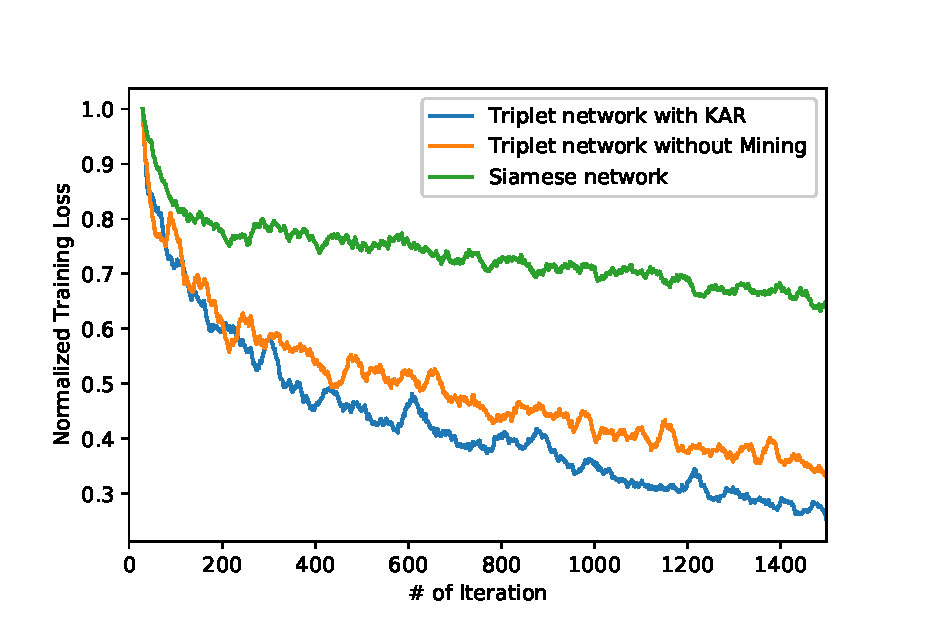
\includegraphics[width=\textwidth]{normalized_loss_curve_ma30_v1.eps}
    \caption{Training Loss Curve of the Proposed System} \label{fig2}
\end{figure}


\section{Conclusion}
In this paper, we proposed an identity verification system based on the handwritten signature signals captured by the Wi-Fi CSI signal using triplet network adopting the kernel and the range (KAR) space learning. 
The kernel and the range space learning is initially adopted to mine the distinctive triple inputs from the training Wi-Fi signature signals. 
Subsequently, the triplet network utilizing the ConvNet structure is trained with the mined triplet inputs based on L-2 distance comparison. 
Our experiments on an in-house Wi-Fi handwritten signature signal dataset showed encouraging verification accuracy with faster training loss convergence compare to the basic triplet network and the Siamese network.
%
% ---- Bibliography ----
%
% BibTeX users should specify bibliography style 'splncs04'.
% References will then be sorted and formatted in the correct style.
%
%\bibliographystyle{splncs04}
%\bibliography{mybibliography}
%


%\begin{thebibliography}{8}

\bibliographystyle{splncs04}
\bibliography{bib_acpr}

%\end{thebibliography}

\end{document}